\documentclass[11pt]{article}

% --- Encoding and fonts ---
\usepackage[utf8]{inputenc}
\usepackage[T1]{fontenc}
\usepackage{lmodern}

% --- Layout ---
\usepackage[a4paper,margin=1in]{geometry}
\usepackage{microtype}
\setlength{\parskip}{0.4em}
\setlength{\parindent}{0pt}

% --- Math, tables, graphics ---
\usepackage{amsmath,amssymb}
\usepackage{booktabs}
\usepackage{array}
\usepackage{tikz}
\usetikzlibrary{arrows.meta,positioning}

% --- Links ---
\usepackage[hidelinks]{hyperref}

% --- Title ---
\title{Trustworthy AI for Foundational Science:\\
A Closed, Audited Human-AI Loop for Machine-Checked Theory Formalization}
\author{Pawe\l{} Kap\l{}a\'nski}
\date{12 June 2026}

\begin{document}
\maketitle

\begin{abstract}
\noindent
Artificial intelligence now proposes hypotheses and even solves open problems, yet most of what
it produces is not machine-checked, so plausible but wrong results threaten to outpace our
capacity to vet them. Proof assistants offer machine-checkable truth, and agentic systems can now
autoformalize and prove mathematics in Lean. A green build is not enough, however: a proof that
compiles can still rest on a vacuous or over-strong axiom. We present a methodology that closes
this gap. A coding agent (Claude Code) is repurposed to formalize a researcher's own new
foundational physics framework in Lean~4 / Mathlib, self-correcting against the compiler; a
second, independent model (GPT-5.5-Pro) adversarially reviews the conceptual design; a human
directs scope and adjudicates; and a soundness audit records which named axioms each result
depends on, ratcheting a tracked budget down and publishing an honest proved/conditional/cited
boundary. A verified blueprint links every human-readable statement to its kernel-checked proof.
Applied to a collapse-free, finite-information account of quantum measurement, the loop drove the
deductive core from fifty-seven project-specific axioms to zero, with no \texttt{sorry}, across
122 modules and roughly 1{,}347 theorems. We report two episodes in which the independent reviewer
caught a false axiom and an inconsistent one that the axiom counter could not see, motivating a
third soundness instrument. We are explicit about scope: verification certifies that the
framework's conditional mathematics is correct and free of hidden axioms, not its physical
postulates, which remain open. The contribution is a transferable architecture for trustworthy
AI-assisted formalization, not a new physical result.

\medskip
\noindent\textbf{Keywords:} AI for science; autoformalization; interactive theorem proving; Lean;
multi-agent systems; LLM-as-judge; verification; soundness auditing; human-AI collaboration.
\end{abstract}

\section{Introduction}

\subsection{The verification crisis in AI-for-science}

In the span of two years, large language models have moved from solving textbook exercises to
operating as research agents. Systems now generate hypotheses, design and run experiments, and
draft papers end to end \cite{r1,r2}, propose research programmes as ``AI co-scientists'' \cite{r3},
and in at least one case derive a novel closed-form result for an open problem in theoretical
physics \cite{r4}. The trajectory is steep, and it is accelerating.

The stakes scale with that velocity. As the cost of generating a plausible-looking scientific
claim falls toward zero, the binding constraint on science shifts from production to verification.
The bottleneck is no longer writing a derivation but establishing that a derivation is correct, and
human refereeing does not scale at the rate machine generation does. A field that produces claims
faster than it can check them accumulates a growing reservoir of unverified results, some fraction
of which are wrong in ways that are expensive to discover later. This is the structural problem the
paper addresses, and it is why the moment calls for a checkable methodology rather than a more
capable generator.

The danger is also specific in form. The great majority of these outputs are expressed in natural
language and are not machine-checked. Language models remain prone to hallucination: fluent
reasoning that is locally plausible and globally wrong \cite{r5}. In ordinary software a flaw of
this kind surfaces as a failing test; in mathematics and theoretical science it can survive review,
because a subtly invalid step is the kind of thing a hurried human referee misses. Recent work
states the consequence plainly. Without rigorous verification, the flood of machine-generated
hypotheses risks overwhelming science with results that look like discoveries but are not
\cite{r6}, and even autonomous-research pipelines stumble where correctness, rather than fluency,
is the binding constraint \cite{r7}.

The most promising answer is to make the machine's reasoning checkable by another machine.
Interactive theorem provers such as Lean~\cite{r38}, with its mathematical library Mathlib~\cite{r39},
reduce ``is this argument correct?'' to ``does the kernel accept this term?'', and a vigorous research front now
trains and scaffolds models to autoformalize informal mathematics and to produce formally verified
proofs \cite{r8,r9,r10}. Formal mathematical reasoning has been argued to be a genuine new frontier
for AI for this reason: it supplies an oracle for correctness that scales without human
refereeing \cite{r11}.

\subsection{Machine-checking plus auditing as the missing filter}

Formal verification is necessary but not sufficient, and the gap between the two is where this
paper lives. A Lean development can compile, contain no \texttt{sorry} placeholder, and still be
unsound as a model of its intended claims, because the load-bearing content has been pushed into an
\texttt{axiom}, a declaration the kernel accepts without proof. Two failure modes follow. An axiom
can be simply false, asserting more than is true, in which case everything downstream is vacuously
``proved.'' Or an axiom can be vacuous or inconsistent (for instance, an implication whose
hypothesis is the trivially-true proposition), in which case it silently trivializes the theorems
that consume it. Neither failure is caught by the two checks practitioners habitually run, ``it
builds'' and ``it has no \texttt{sorry}.'' A development can pass both and rest on a contradiction.

The corrective is to treat the axiom base itself as a first-class object of audit. For each result
the paper relies on, one can ask the proof assistant to print the exact set of axioms the result
transitively depends on, classify each as a standard logical axiom, a named domain assumption, or
an external citation, and track how that set changes over the life of the project. Done
consistently, this converts ``the proof compiles'' into the stronger and more honest statement
``here is precisely which assumptions the result rests on, and here is the trajectory by which that
set shrank.'' We call this discipline soundness auditing, and we argue that it is the missing
companion to machine-checking for trustworthy AI-assisted science.

\begin{center}
\fbox{\begin{minipage}{0.93\linewidth}
\textbf{What we claim, and what we do not.} We claim a transferable methodology (a human-directed,
two-model loop with an explicit, shrinking axiom audit and a verified human-readable bridge),
together with an existence proof that it scales to a complete theory. We do not claim that AI
discovered or proved new physics; the case-study theory's physical postulates remain open
(\S4.3, \S5.3). The proved/conditional/cited boundary is maintained throughout, and the central
honesty principle is that an axiom-free development in the proof assistant certifies the
conditional mathematics, not the physics.
\end{minipage}}
\end{center}

The thesis of the paper, in one sentence: for AI to contribute trustworthily to foundational
science, ``the proof compiles'' must be replaced by ``here is exactly which named axioms the result
depends on,'' and we exhibit a human-directed, two-model loop that delivers this by formalizing a
new collapse-free quantum-measurement theory end to end with a continuously audited, ratcheting
axiom budget that reached zero for the deductive core.

\subsection{Contributions}

\begin{itemize}
\item \textbf{A closed, audited human-AI formalization loop.} A coding agent that formalizes and
  self-corrects against the Lean compiler, an architecturally independent model that adversarially
  reviews the conceptual design, and a human who sets scope and adjudicates. The organizing idea is
  a division between mechanical correctness (owned by the compiler) and conceptual soundness (owned
  by the reviewer and the audit), described in \S3.2 to \S3.4.
\item \textbf{An axiom-budget discipline as a soundness instrument.} A continuously maintained,
  CI-enforced audit that prints and classifies the axiom dependencies of every headline result,
  ratchets a budget downward, and publishes the proved/conditional/cited split (\S3.5).
\item \textbf{An existence proof at the scale of a whole theory.} End-to-end formalization of a
  researcher's own new foundational framework, not a benchmark and not a published lemma, driving
  its deductive core from 57 project axioms to 0, with no \texttt{sorry}, over 122 modules and
  about 1{,}347 theorems (\S4).
\item \textbf{Two documented soundness saves and a third instrument.} Two concrete,
  kernel-checkable episodes in which the independent reviewer caught a false axiom and an
  inconsistent one invisible to the axiom counter, which motivated a vacuity lint as a complementary
  guard (\S4.4).
\item \textbf{A verified human-readable bridge.} A blueprint whose formalized tags are mechanically
  linked to kernel-checked declarations, making an AI-formalized result auditable by domain experts
  who do not read Lean (\S3.6).
\item \textbf{A reproducible artifact.} A public repository, the axiom audit, and the blueprint, so
  that every claim in \S4 is checkable down to its proof.
\end{itemize}

\subsection{Roadmap}

Section~2 situates the work against autoformalization and agentic proving, AI-for-science,
LLM-as-judge, and physics-in-Lean. Section~3 specifies the loop, the audit, the blueprint bridge,
and the reproducibility protocol. Section~4 reports the case study with metrics, the discharge
trajectory, and the two reviewer-caught episodes. Section~5 discusses what generalizes, the failure
modes, and the threats to validity. Section~6 concludes.

\section{Related Work}

Four lines of work bound the contribution. We review each and state where the present method
departs from it. The recurring pattern is that each line solves a piece of the problem (proving
given theorems, generating hypotheses, judging outputs, or formalizing settled physics), but none
combines the four ingredients we do: formalizing a researcher's own new theory, an independent
adversarial reviewer inside the verifier loop, an axiom-level soundness audit, and a verified
human-readable bridge.

\subsection{Agentic autoformalization and theorem proving}

Autoformalization, the translation of informal mathematics into a proof assistant's language, was
established as an LLM-era programme by Wu et al.\ \cite{r8} and given an influential method in
Draft-Sketch-Prove, which drafts an informal proof, sketches a formal skeleton, and closes the gaps
with a prover \cite{r9}; a recent survey maps the now-substantial field \cite{r10}. Agentic systems
add tool use and self-correction against the verifier. Ax-Prover pairs LLM reasoning with Lean tools
over the Model Context Protocol and proves theorems across abstract algebra and quantum theory, and
it assisted experts in machine-checking an entropy bound from quantum key distribution \cite{r12}.
LeanMarathon targets long-horizon autoformalization with a multi-agent harness designed for
legibility and drift-resistance \cite{r13}. Multi-agent generate-and-repair loops and
verifier-guided iteration improve reliability on benchmarks \cite{r14,r15}, and dedicated systems
learn to repair Lean proofs from compiler feedback \cite{r16}.

The defining feature of this line is that the target theorems are externally given: competition
problems, benchmark suites, or statements lifted from existing papers. The soundness question is in
a sense pre-settled, because the statement's correctness is not in doubt, only its proof. Our work
differs in kind. The target is a researcher's own, still-contested theory, where the danger is not
a wrong proof of a right statement but a right proof of a wrong-because-vacuous statement, or a
proof that quietly assumes its conclusion. An externally fixed target excludes that danger; an
own-theory target invites it, which is why the audited loop, rather than the prover, is our
contribution. This line shares our self-correction mechanism (the formalizer working against the
compiler, \S3.2), but it does not pair that mechanism with an independent conceptual reviewer or an
axiom audit.

\subsection{AI-for-science and autonomous discovery: the verification gap}

A parallel line builds agents that conduct research. The AI Scientist and its successor automate
machine-learning discovery, including writing and a measure of automated reviewing \cite{r1,r2};
AI co-scientist and collaborative-research platforms generate and triage hypotheses \cite{r3};
experience reports and surveys catalogue the emerging practice \cite{r17,r18}. A neuro-symbolic
system recently solved an open problem in theoretical physics, deriving exact analytic solutions for
a gravitational-radiation power spectrum \cite{r4}, but it did so through tree search and numerical
feedback, with no formal theorem prover in the loop, so the result's correctness rests on numerical
agreement rather than machine-checked deduction. Sober assessments document where such pipelines
fail \cite{r7}, and the verification-gap critique \cite{r6} is, in effect, the motivation for the
present paper. This line shares our ambition of engaging real research questions rather than
benchmarks, but it typically forgoes machine-checking, and where it includes automated review, that
review evaluates generated papers, not formal-proof soundness. We keep the ambition and add both the
proof assistant and the audit.

\subsection{LLM-as-judge and adversarial review}

The idea of using one model to evaluate another is now well studied. Surveys of agent-as-a-judge
evaluation \cite{r19}, multi-agent debate among judges with stability analysis \cite{r20},
meta-judge frameworks \cite{r21}, analyses of bias under many-minds judging \cite{r22}, and methods
that audit reasoning trees rather than vote \cite{r23} establish that a separate critic can improve
reliability, and that independence and diversity of vantage are what make the critique informative.
We take that finding and relocate it. This literature studies judging in the abstract, scoring
free-standing outputs against a rubric. Our reviewer instead sits inside a verifier-backed
formalization pipeline, where mechanical correctness is already guaranteed by the compiler, so the
reviewer's remit is narrowed to what the compiler cannot see: vacuous hypotheses, over-strong or
false axioms, hidden circularity, and prose that overclaims relative to the Lean. Its output is not
a score but a set of design critiques fed back into the loop under human adjudication. The two
documented saves of \S4.4 are evidence that an independent reviewer, so positioned, catches
soundness faults that a single capable agent does not.

\subsection{Formalizing physics in Lean}

Bringing proof assistants to physics is nascent but active. A landmark effort formalized the
construction of free bosonic quantum field theory and its Osterwalder-Schrader/Glimm-Jaffe axioms
in Lean~4 / Mathlib, explicitly as a proof of concept that extended mathematical-physics arguments
can be machine-checked with current AI tools \cite{r24}; the generalized quantum Stein's lemma has
been formalized \cite{r25}; PhysProver and the PhysLean effort build datasets, tactics, and tooling
for physical theorems \cite{r26,r27}, with index-notation infrastructure \cite{r28} and earlier
chemical-physics work \cite{r29}; and a recent perspective surveys the state of interactive theorem
provers in physics \cite{r30}. These efforts target settled results: theorems with accepted proofs,
digitized into Lean. The foundations and interpretation of quantum mechanics, the measurement
problem, where the contribution is conceptual and contested and the premises are exactly what is in
dispute, has not been a target. It is the domain of our case study, and it is the setting in which
the audit proves its worth, because a contested foundational claim is where an unnoticed vacuous or
over-strong assumption can masquerade as a result.

\section{Method: A Closed, Audited Human-AI Formalization Loop}

\subsection{Architecture overview}

The method is a loop among four roles (Figure~\ref{fig:loop}). A human sets the target and the
admissible assumptions, and adjudicates. A formalizer, which is a coding agent, writes Lean and
self-corrects against the compiler until the build is green. The resulting development is read by an
adversarial reviewer, a second and independent model, whose job is to attack the design rather than
the syntax. An axiom auditor extracts from the kernel the axioms that each headline result depends
on, and a CI guard enforces a non-increasing budget. A blueprint renders the result in ordinary
mathematics with every statement linked to its proof. The organizing principle is a separation of
concerns: mechanical correctness is delegated to the compiler; conceptual soundness is delegated to
the reviewer and the audit; and the human owns scope and the gatekeeping of premises.

\begin{figure}[ht]
\centering
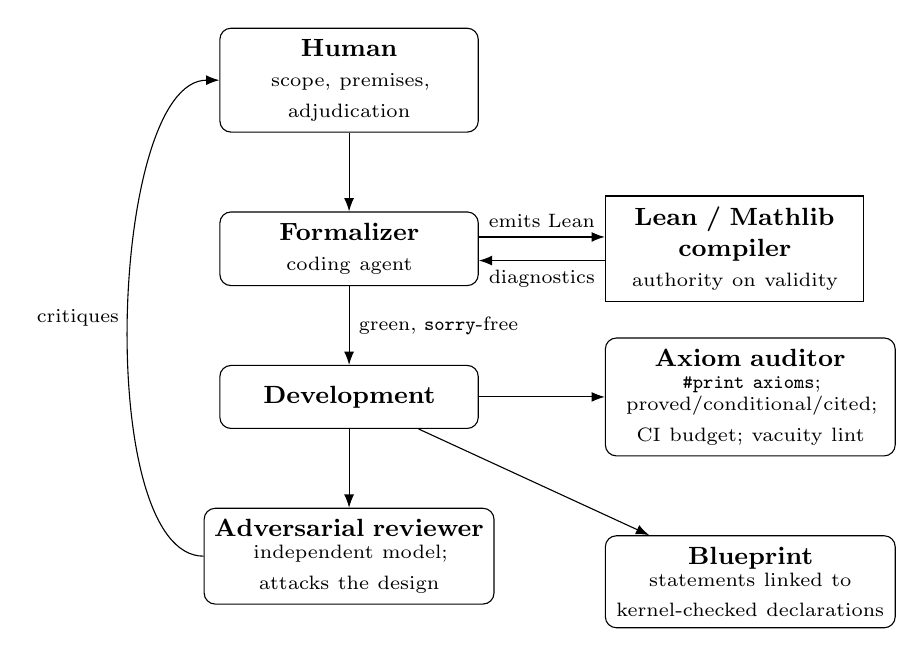
\begin{tikzpicture}[
  >=Latex, node distance=10mm and 16mm,
  box/.style={draw, rounded corners, align=center, inner sep=4pt, font=\small,
              minimum height=8mm, text width=30mm},
  oracle/.style={draw, align=center, inner sep=4pt, font=\small,
                 minimum height=8mm, text width=30mm},
  lbl/.style={font=\scriptsize, midway}
]
\node[box] (human) {\textbf{Human}\\\scriptsize scope, premises, adjudication};
\node[box, below=of human] (form) {\textbf{Formalizer}\\\scriptsize coding agent};
\node[oracle, right=of form] (comp) {\textbf{Lean / Mathlib}\\\textbf{compiler}\\\scriptsize authority on validity};
\node[box, below=of form] (dev) {\textbf{Development}};
\node[box, right=of dev, text width=34mm] (aud) {\textbf{Axiom auditor}\\\scriptsize \texttt{\#print axioms};\\proved/conditional/cited;\\CI budget; vacuity lint};
\node[box, below=of dev, text width=34mm] (rev) {\textbf{Adversarial reviewer}\\\scriptsize independent model;\\attacks the design};
\node[box, below=of aud, text width=34mm] (bp) {\textbf{Blueprint}\\\scriptsize statements linked to\\kernel-checked declarations};

\draw[->] (human) -- (form) node[lbl,right]{};
\draw[->, transform canvas={yshift=1.5mm}] (form) -- (comp) node[lbl,above]{\scriptsize emits Lean};
\draw[<-, transform canvas={yshift=-1.5mm}] (form) -- (comp) node[lbl,below]{\scriptsize diagnostics};
\draw[->] (form) -- (dev) node[lbl,right]{\scriptsize green, \texttt{sorry}-free};
\draw[->] (dev) -- (aud);
\draw[->] (dev) -- (rev);
\draw[->] (dev) -- (bp);
\draw[->] (rev.west) .. controls +(left:14mm) and +(left:14mm) .. (human.west)
      node[lbl,left,pos=0.5]{\scriptsize critiques};
\end{tikzpicture}
\caption{The closed, audited loop. The compiler is the authority on mechanical correctness; the
reviewer and the axiom audit address conceptual soundness; the human owns scope and premise
control.}
\label{fig:loop}
\end{figure}

\subsection{The formalizer: a coding agent with compiler self-correction}

The formalizer is a general-purpose coding assistant, repurposed so that its output language is Lean
rather than software and its oracle is the Mathlib build rather than a test suite. In practice this
is a tight inner loop. The agent proposes a definition or a proof term, invokes the build, reads the
diagnostics (an unsolved goal, a type mismatch, an unknown identifier, a failed tactic), and
revises, iterating until the kernel accepts the increment. The diagnostics are unusually informative
compared with a failing software test, because Lean reports the exact remaining goal state, which
functions as a precise specification of what is still to be proved, so the agent's search is guided
rather than blind. Two disciplines make this reliable. The first is to ship green increments: each
unit of work ends with a compiling, \texttt{sorry}-free addition, committed to version control only
when the kernel accepts it, so the development never carries an unproved gap labelled as proved. The
second is to allow no silent \texttt{sorry}: the placeholder that lets Lean accept an unproved
statement is treated as a build failure by policy, not a convenience, so the agent cannot make
progress by deferring a hard step. Mechanical correctness is therefore continuous and
non-negotiable, and it is delegated entirely to the compiler. The agent is never the authority on
whether a proof is valid.

What the formalizer is not good at is what the rest of the loop supplies. Faced with a hard lemma it
cannot close, the agent's path of least resistance is to introduce an \texttt{axiom}, a declaration
the kernel accepts without proof, and to proceed. This is legitimate as a temporary interface, but
it is also where unsoundness enters, because the agent has little incentive, and limited ability, to
notice that the axiom it wrote is false, vacuous, or assumes the very thing downstream theorems will
``prove.'' The audit (\S3.5) makes every such axiom visible, and the reviewer (\S3.3) attacks it.

\subsection{The adversarial reviewer: an independent model critiquing design}

Compiler-checking guarantees that a proof is valid. It is silent on whether the statement is the
intended one, whether a convenient axiom smuggles in the conclusion, and whether the surrounding
prose claims more than the Lean delivers. These are conceptual judgments, and a single agent is poor
at them about its own work, because the commitments that produced a design are the same commitments
that hide its flaws from the inside, and an agent that has just spent effort making a module compile
is inclined to regard it as finished. We therefore assign conceptual review to a different model
(GPT-5.5-Pro) with a different training lineage, invoked after each significant step rather than only
at the end, so that a flawed design is caught before downstream work is built on it.

The reviewer's prompt is adversarial. It is asked to find hypotheses that are vacuous or trivially
satisfiable, meaning an antecedent that constrains nothing; to find axioms that are over-strong or
simply false, and to attempt an explicit counterexample; to find circular dependencies, where a
result is used, directly or transitively, in establishing one of its own premises; and to find
places where the natural-language statement of a theorem, or the paper's description of it,
overclaims relative to the formal content. The reviewer is not asked to check proof validity. That
is the compiler's job, and asking a language model to do it would reintroduce the unreliability the
proof assistant removes. Its remit is narrowed to the soundness questions the compiler cannot
answer. Its critiques are advisory rather than authoritative: the human adjudicates, and the reviewer
is sometimes wrong in both directions (\S5.2). But it is independent, and independence of vantage,
the property the LLM-as-judge literature identifies as the source of value \cite{r19,r22}, surfaces
the failure modes the formalizer cannot see in itself. Section~4.4 documents two cases in which this
independence was decisive.

\subsection{Human direction: scope, adjudication, premise control}

The human is not eliminated, and the paper does not pretend otherwise. The contribution is a division
of labour that concentrates scarce human judgment, not a claim of autonomy. Three responsibilities
are irreducibly human in our setup. The first is scope: choosing which results to attempt and in what
order, including the strategic decision of which conjectures are worth the cost of formalization and
which are better left as cited frontier. The second is premise control: deciding which assumptions
may enter as a named axiom, and which must be proved outright or recast as an explicit hypothesis on
the theorems that use them. This is the most consequential lever over soundness, because it
determines what the audit will later expose and what the budget will count; converting a tempting
axiom into an explicit hypothesis is the standard way a hidden assumption is brought into the open,
and it reappears in \S4.4, Case~2. The third is adjudication: resolving disagreements between the
formalizer and the reviewer, deciding when a critique warrants a redesign rather than a
clarification, and ruling on whether a proposed statement faithfully captures the intended claim. The
value of the method is that it routes the two models' output through these decisive human decisions
while delegating mechanical proof search to the formalizer and first-pass conceptual critique to the
reviewer, so the human spends attention on premises and adjudication rather than on proof
bookkeeping.

\subsection{Soundness instrumentation: the axiom budget and proved/conditional/cited audit}

The audit is central to the trust claim, and it works because modern proof assistants expose their
own trusted base. In Lean, the command \texttt{\#print axioms F} reports the exact set of axioms that
the term \texttt{F} transitively depends on, computed by the kernel rather than by inspection of the
source, so nothing a proof uses can escape it. We maintain a dedicated audit module containing such a
directive for every headline theorem (795 of them in the case study), and we classify each dependency
into three buckets. A result is proved when its axiom set contains only the standard logical axioms of
the system, which for Lean are \texttt{propext}, \texttt{Classical.choice}, and \texttt{Quot.sound},
the axioms that every ordinary theorem in the library uses and that we do not count against the
project. It is conditional when it additionally depends on a named domain assumption that the project
introduced as an \texttt{axiom}; each such assumption is listed, with a statement of what it asserts
and why it is not yet proved. It is cited when the surrounding argument appeals to an external result
that is not formalized here at all, such as a continuum theorem available only in the literature. The
project-specific axioms, the conditional bucket, are counted into a single budget.

Two policies turn this from a report into an instrument. First, a continuous-integration guard fails
the build if the count of project-specific axioms rises without an accompanying written justification,
so the budget can only ratchet down over time; an analyst who wants to add an assumption must say so,
on the record. Second, a companion document narrates the discharge of each axiom, recording what it
asserted and the theorem or construction that replaced it, so the audit is a verifiable history rather
than only a number. The boundary between what is established and what is assumed is thereby made
machine-checked and public, and its movement becomes an observable quantity. When that boundary's
project-axiom count reaches zero, the statement ``the deductive core rests on no assumption beyond
standard logic'' is not a claim to be trusted but a CI result anyone can reproduce.

One subtlety, which \S4.4 shows is not hypothetical, is that the axiom count is blind to a vacuous or
inconsistent axiom. A declared assumption whose hypothesis is trivially true contributes one to the
count while constraining nothing, and removing it lowers the count without improving soundness; the
inconsistency it introduced was the real problem. The budget therefore needs a companion that
inspects axiom content, not only cardinality, a point we return to in \S3.7 and \S4.4.

\subsection{The verified blueprint bridge}

An AI-formalized theory that only Lean experts can read fails the people who must evaluate it, here
physicists, who will not and should not be asked to audit proof terms. We therefore maintain a
blueprint: a document of ordinary mathematical statements in which each statement is annotated with
the name of the Lean declaration that proves it. A checker, run in continuous integration, verifies
that every such name resolves to a real, kernel-checked declaration in the build, so the human-readable
exposition cannot silently drift from the formal development; if a referenced declaration is renamed
or removed, the check fails. A dependency graph renders the logical structure of the development, with
each node coloured according to whether its statement, and its proof, are formalized, so a reader sees
at a glance which parts of the narrative are backed by the kernel and which are still prose.

Earlier tools generate blueprints as a one-off export \cite{r31,r44}; the artifact here is instead an
integral, continuously-verified bridge. A formalized tag in the human-readable document is necessarily
backed by a proof the kernel accepts, and the link is maintained in CI alongside the build and the
audit. This lets a domain expert read the mathematics in their own language while retaining the
guarantee that it matches what was proved, and it is a concrete answer to the objection that
AI-generated technical content cannot be trusted: every claim in the exposition is clickable down to a
machine-checked proof, and the linkage itself is checked.

\subsection{Protocol and reproducibility}

A round of the loop runs as follows. First, the human fixes a target result and the set of premises
that may be assumed for it. Second, the formalizer produces a compiling, \texttt{sorry}-free
increment, iterating against the compiler as in \S3.2. Third, the axiom auditor records the
increment's axiom dependencies via \texttt{\#print axioms} and updates the budget, and a vacuity lint
scans the new code for trivially-true hypotheses and vacuous propositional bodies, complementing the
count with a check on axiom content. Fourth, the adversarial reviewer critiques the design along the
four axes of \S3.3. Fifth, the human adjudicates, either accepting the increment, ordering a redesign,
or converting an axiom into an explicit hypothesis on the consuming theorems. Role boundaries are
fixed and do not blur: the compiler is the sole authority on proof validity; the reviewer never edits
proofs and never has the last word; the human alone admits an axiom into the budget.

Reproducibility is built in rather than asserted. The full development, the per-theorem audit module,
the budget-check and vacuity-lint scripts, and the blueprint are published in a public repository at a
pinned commit. Every metric in \S4 is therefore independently checkable. The project-axiom count is a
one-line query over the source that anyone can run; the build status and the absence of \texttt{sorry}
are the continuous-integration result; the vacuity-lint outcome is a script; and the blueprint's
claim-to-proof links are verified by the bundled checker. We regard this property, that the paper's
quantitative claims about its own soundness can be re-derived from the artifact rather than taken on
faith, as part of the methodology rather than an afterthought to it.

\section{Case Study: Formalizing a Collapse-Free Quantum Measurement Theory}

The target theory, QIQT-H, is a foundations-of-physics framework that we treat strictly as a
formalization target, not as a claim to defend. We describe it neutrally, then report what the loop
produced and what it did not.

\subsection{The target theory, in neutral terms}

QIQT-H is a single-world, exactly-unitary account of quantum measurement. Its premise is that the
physical instantiation of a wave function in a bounded spacetime region carries only finite
information, bounded by a holographic capacity \cite{r40}. Together with environmental decoherence,
this is argued to make multi-record macroscopic states non-instantiable, so that a single definite
record obtains per run, with a non-dynamical actuality selector fixing which record, and the Born
rule appearing as an across-run frequency rather than a per-run probability \cite{r32,r33,r34}. The
proposal continues a finite-information line of approaches to measurement \cite{r41}; it is set out
in a companion paper \cite{r42}, and the Lean development we report on is public \cite{r43}. Whether
these physical claims are true is not our subject. Our subject is whether the framework's deductive
core can be formalized end to end, honestly audited, and rendered legible. The framework's own authors
flag its central physical postulates as open, and the formalization respects that boundary exactly.

\subsection{What was formalized, with artifact metrics}

The development formalizes the framework's layered deductive core, and it is worth naming the layers
because their epistemic shapes differ and the method's job is to keep those differences explicit. A
first layer mechanizes the no-collapse mechanism. From a finite additive capacity and a
redundant-record (Spectrum Broadcast) structure \cite{r45}, it derives that at most one macroscopic
record can be co-instantiated, with the capacity threshold itself derived from orthonormality rather
than stipulated, and a per-collision distinguishability derived from a textbook interaction
Hamiltonian. A second layer treats the Born rule as a conditional representation theorem. An
effect-Gleason argument \cite{r35,r36} shows that a positive, normalized, non-contextual outcome
assignment must be the Born functional, and
a join assembles unique actual histories carrying the Born product law under explicit
product-preparation and non-contextuality hypotheses. This layer is accompanied by a deliberate suite
of negative results: that linear unitary decoherence does not concentrate branch weights, that the
structural axioms do not single out Born among distributions, that support preservation is strictly
weaker than Born equivariance \cite{r37}, and that operational click-statistics underdetermine the
underlying measure. Together these establish that the conditional theorem's premises are necessary rather than
decorative. A third layer lifts the finite marginals to a covariant, $\sigma$-additive typicality
measure over global measurement histories via a Kolmogorov-style extension, state-agnostically, with
an operational no-signaling result for arbitrary entangled states. A fourth layer discharges the
abstract normal-state input with a genuine normal state on the algebra of bounded operators and
exhibits a free-field, boost-invariant instance. Above these sits a continuum tower, comprising
bounded spectral theory and projection-valued measures, Fock space and Weyl/CCR structure, and the
entropy and data-processing machinery; it is under construction toward the framework's open problems
and is not yet complete.

Naming the layers matters because the audit treats them uniformly. Every theorem above, across all
four layers and the in-progress tower, is subject to the same \texttt{\#print axioms} discipline, and
every one of them, including the negative audits, which are themselves theorems that something does
not follow, lands in the proved bucket.

The artifact is quantified rather than asserted. As of 2026-06-12 the development comprises 122 modules
and approximately 1{,}347 theorems and lemmas, with 795 \texttt{\#print axioms} directives in a
dedicated audit module. It builds green, contains no \texttt{sorry}, and depends on zero
project-specific axioms, so every audited theorem rests only on the three standard Lean axioms. A
vacuity scan (\S4.4) reports a single benign site. Table~\ref{tab:metrics} summarizes.

\begin{table}[ht]
\centering
\caption{Artifact metrics (verified 2026-06-12).}
\label{tab:metrics}
\begin{tabular}{@{}ll@{}}
\toprule
Quantity & Value \\
\midrule
Lean modules & 122 \\
Theorems / lemmas & $\sim$1{,}347 \\
\texttt{\#print axioms} directives (audit) & 795 \\
Project-specific axioms & 0 \\
\texttt{sorry} occurrences & 0 \\
Vacuity-lint sites & 1 (benign; an indiscrete-preorder definition) \\
Build status & green \\
\bottomrule
\end{tabular}
\end{table}

\subsection{The audit in action: the ratchet, and the honesty boundary}

The audit's signal is a trajectory rather than a single number. Over the project's life the count of
project-specific axioms fell
\[
 57 \to 40 \to 37 \to 35 \to 33 \to 32 \to 31 \to 29 \to 21 \to 17 \to 8 \to 7 \to 6 \to 0.
\]
The ratchet is honest about its own shape. Several passes raised the count, introducing a named
interface axiom to make a new conditional result explicit before later discharging it; the budget
measures exposed assumptions, and exposing one is progress over hiding it inside a proof. The
discharges are not bookkeeping, because each replaced an assumption with mathematics. An eleven-axiom
relative-entropy interface, comprising the abstract properties of Araki relative entropy on which the
framework's entropy arguments depended, including Donald's identity and the Holevo bound
$\chi \le H(p)$, was discharged to theorems by realizing the interface in a finite-dimensional matrix
model and proving the Holevo bound pointwise via operator-monotonicity of the logarithm, transported
through a bridge to C*-matrix structure. An eight-axiom packaging of Donald's identity was likewise
replaced by a typeclass with a concrete, axiom-free instance, as were a four-axiom
data-processing-inequality interface, realized by a concrete mixed-unitary channel, and a
relative-entropy-positivity (Klein) interface. On the Born side, a Goldstein-Struyve ``Schur
classification'' that had stood as a named axiom was proved outright, as was the attainability half of
the Tsirelson bound by an explicit construction; and the effect-Gleason capstone, that positivity,
normalization, and ray-certainty force the Born functional, was proved, retiring the false axiom of
\S4.4. The endpoint is that the deductive core depends on no project-specific axiom at all: every one
of the former interface assumptions is now either a theorem in a concrete realization or an explicit
hypothesis on the theorems that use it.

Three layers must be held apart, and the audit holds them apart (Table~\ref{tab:layers}). The
deductive core is axiom-free. The framework's physical postulates, namely the holographic
instantiation bound, the macroscopic-definiteness conjecture, the canonical typicality (Born)
principle, and the Lorentz covariance of the selector, are open, and an axiom-free Lean development
bears on none of them. A continuum formalization frontier is in progress. The most important sentence
of this section is therefore the following: an axiom-free development in the proof assistant certifies
that the framework's conditional mathematics is correct and rests on no hidden axiom; it does not
establish the physics. We repeat this guard in \S5.3.

\begin{table}[ht]
\centering
\caption{The three-layer status boundary.}
\label{tab:layers}
\begin{tabular}{@{}p{0.46\linewidth}p{0.46\linewidth}@{}}
\toprule
Layer & Status (2026-06) \\
\midrule
Conditional/structural deductive core & Machine-checked, axiom-free (standard axioms only) \\
Physical postulates (capacity bound; definiteness; Born; covariance) & Open; not theorems; unaffected by formal discharge \\
Continuum realization (Type~II / Fock / modular flow) & Formalization frontier, in progress \\
\bottomrule
\end{tabular}
\end{table}

\subsection{What the reviewer caught: two soundness saves}

The value of the loop is not that it produced a compiling development, since many systems do that, but
that it produced an audited one, with documented saves the compiler alone would have missed. Both
episodes below are kernel-checked in the published development, so the reader need not take them on
trust.

\textbf{Case 1, a false axiom.} The formalizer initially encoded a Gleason-type step as a named axiom:
that a normalized, additive, homogeneous valuation on quantum effects that is certain on the state's
ray must equal the Born functional. The independent reviewer, on its third pass over the module,
flagged the axiom as false, because it omits positivity. The refutation, which was then itself
formalized, is a two-dimensional weight that satisfies every stated premise yet is not the Born
functional. The false axiom was retired and replaced not by a patch but by proved content: a lemma
deriving ray-support from positivity, and a capstone showing that a positive, normalized, ray-certain
weight is the Born functional. The fix made the result stronger, since Born now follows from
positivity, an honest hypothesis, and it removed an axiom. The lesson is that an independent vantage
catches a capable agent's plausible-but-false premise.

\textbf{Case 2, an inconsistent axiom the counter could not see.} A locality interface was encoded as
an axiom whose hypothesis was the trivially-true proposition. Because a \texttt{True} antecedent
constrains nothing, the axiom in effect asserted a universal equality that is simply false, and any
theorem consuming it inherited an inconsistency. Neither of the habitual checks detects this: the
development builds, and it contains no \texttt{sorry}, yet it rested on a contradiction. The axiom was
removed, and the affected theorem now takes locality as an explicit hypothesis, relocating the
assumption into the open. In response, the project added a third soundness instrument, a vacuity lint
that scans for vacuous propositional bodies and trivially-true antecedents, to complement the axiom
counter. It currently reports a single site, which inspection confirms is a legitimate
indiscrete-preorder definition rather than a hidden assumption. This episode captures the paper's
central point: ``compiles, no \texttt{sorry}, axiom count zero'' is necessary but not sufficient, and
soundness requires auditing for vacuity and inconsistency as well.

Taken together, and set against the trajectory ending at zero, the two cases are the empirical payload.
The loop did not merely yield a green build; it yielded an audited, shrinking-to-zero conditional base
with concrete, checkable saves.

\section{Discussion, Limitations, and Threats to Validity}

\subsection{What generalizes, and how to port it}

The loop and the audit are domain-agnostic. Nothing in \S3 is specific to physics or to the particular
case-study theory. The construction is a self-correcting formalizer, an independent adversarial
reviewer, a \texttt{\#print axioms}-based proved/conditional/cited audit with a ratcheting budget, a
vacuity lint on axiom content, and a verified blueprint. Any formalization effort in which soundness,
not merely compilation, matters can adopt it.

To make the transfer concrete, consider porting the loop to a different domain, say the verification
of a novel cryptographic protocol's security argument, or a new result in distributed-systems theory.
The steps are mechanical. (i)~Choose the proof assistant and library that already cover the most
background, whether Lean/Mathlib, Isabelle/HOL, or Coq, so the formalizer spends its effort on the new
content rather than on rebuilding foundations. (ii)~Have the human decompose the target into a
deductive core, meaning what should be proved, and a cited frontier, meaning results to assume from the
literature, and fix, per result, which premises may be axioms. (iii)~Run the inner
formalize-and-self-correct loop to a green, \texttt{sorry}-free state. (iv)~After each module, emit the
axiom audit, classify proved/conditional/cited, and run the vacuity lint. (v)~Have an independent model
adversarially review the design for vacuity, over-strong axioms, circularity, and overclaiming.
(vi)~Maintain a blueprint linking each human-readable claim to its checked declaration. The only
domain-specific inputs are the target decomposition and the premise policy, both human and both
decisive, and the rest is the same instrument. The pattern is most valuable where the cost of a hidden
assumption is highest: original theories, contested foundations, and safety-relevant or
security-relevant claims, where ``it compiles'' is the reassurance one must not accept uncritically. It
is least valuable for routine benchmark proving, where the target is externally certified and the
soundness question is already settled.

\subsection{Failure modes and the human's irreducible role}

The method is not autonomous and we do not present it as such, and its failure modes are as important
to report as its successes. The formalizer stalls on genuinely hard lemmas and, often, on gaps in the
underlying library, where a result it needs is simply not in Mathlib and supplying it is a research
task in its own right rather than a matter of search. In such cases the agent's tempting shortcut is to
introduce an axiom, which is why the audit and the reviewer must be running: an unsupervised formalizer
left to clear its own blockers will accumulate assumptions. The reviewer is sometimes wrong in both
directions. It is over-cautious when it flags a sound construction as suspicious, which is common when a
definition is unusual but correct, and over-confident when it pronounces a module clean that in fact
harbours a subtle problem; we observed both. Its value is therefore statistical and adversarial rather
than oracular: it raises candidates, and the human and the compiler dispose of them. Finally, the human
remains the premise gatekeeper, which is the load-bearing role. The audit makes assumptions visible,
but visibility is not acceptability, and a human still decides which assumptions a result may rest on.
The honest claim is that the loop concentrates scarce human judgment onto premise control and
adjudication and removes it from proof bookkeeping, not that it removes the human.

\subsection{Threats to validity}

Several limits bound the strength of our conclusions. The first is that this is a single case study:
we report one theory, one team, one toolchain, so the method's generality is argued rather than
demonstrated across independent efforts, and multi-team replication is needed. The second is model and
version specificity: the results depend on particular models and their versions, and the qualitative
behaviour, especially the reviewer's catch rate, may shift as models change. The third is audit
completeness: the audit certifies which axioms a result depends on and that none are vacuous by the
lint's criteria, but ``no vacuous axiom the lint can see'' is weaker than ``every assumption is
justified,'' and a sufficiently subtle mis-formalization of a statement, as opposed to a proof, remains
possible in principle, which is part of why the blueprint bridge and human review matter. The fourth,
and most important, is that the case-study theory's own physics is not closed by formalization: driving
the deductive core to zero axioms says nothing about whether the holographic capacity bound, the
definiteness conjecture, or the Born principle are physically correct. We state this not as a closing
caveat but as a structural feature of what machine verification can and cannot do for foundational
science.

\section{Conclusion}

AI can now do an alarming amount of science, and very little of it is checkable. We have argued that
the answer is not only to machine-check AI-produced reasoning but to audit its axiom base, because a
proof that compiles can still rest on an assumption that is false, vacuous, or question-begging, and
the two checks practitioners habitually run, ``it builds'' and ``it has no \texttt{sorry},'' cannot
tell the difference. We have presented a concrete, transferable instrument for closing that gap: a
human-directed loop in which a self-correcting formalizer is paired with an architecturally
independent adversarial reviewer and a continuously maintained, CI-enforced soundness audit, with a
verified blueprint that makes the result legible to the domain that must judge it.

Applied to a new, contested foundations-of-physics framework, the loop drove the deductive core from
fifty-seven project-specific axioms to zero, with no \texttt{sorry}, across 122 modules and roughly
1{,}347 theorems, and it produced two documented, kernel-checkable soundness saves: a false axiom that
the reviewer refuted by counterexample, and an inconsistent one that the axiom counter structurally
could not see, the second of which motivated a third instrument, a vacuity lint on axiom content. The
contribution is the audited methodology together with the existence proof that it scales to a whole
theory, held throughout under an explicit and repeated honesty boundary: the formalization certifies
that the framework's conditional mathematics is correct and free of hidden axioms; it does not, and
cannot, establish the framework's physical postulates, which remain open.

Three near-term directions follow. The first is independent multi-team replication, since the strongest
test of a methodology is that others can run it, and the artifact is published so they can. The second
is partial automation of the audit and the reviewer protocol, including richer detection of vacuity,
inconsistency, and circularity than a count and a syntactic lint provide. The third is a careful study
of when the independent reviewer adds value, meaning under what conditions its catch rate justifies its
cost, so that human attention is spent where it is decisive. The broader claim we wish to defend is
modest, and we think it is important for the moment AI-for-science is entering: AI-assisted
formalization is most trustworthy not when it proves the most, but when it is most honest, and most
precisely auditable, about exactly what it has and has not assumed.

\section*{Acknowledgements}

The formalization was carried out with Claude Code (Anthropic) as the formalizer and GPT-5.5-Pro
(OpenAI) as the independent adversarial reviewer, under the author's direction. This AI assistance is
the subject of the paper and is disclosed in full in \S3. The development builds on Lean~4 and the
Mathlib library and on the broader interactive-theorem-proving community.

\begin{thebibliography}{99}

\bibitem{r1} C.~Lu et al. \emph{The AI Scientist: Towards Fully Automated Open-Ended Scientific Discovery.} arXiv:2408.06292, 2024.
\bibitem{r2} Y.~Yamada et al. \emph{The AI Scientist-v2: Workshop-Level Automated Scientific Discovery via Agentic Tree Search.} arXiv:2504.08066, 2025.
\bibitem{r3} J.~Gottweis et al. \emph{Towards an AI Co-Scientist.} arXiv:2502.18864, 2025.
\bibitem{r4} M.~P.~Brenner, V.~Cohen-Addad, and D.~Woodruff. \emph{Solving an Open Problem in Theoretical Physics using AI-Assisted Discovery.} arXiv:2603.04735, 2026.
\bibitem{r5} M.~Liu and J.~Fang. \emph{Enhancing Mathematical Reasoning in Large Language Models with Self-Consistency-Based Hallucination Detection.} arXiv:2504.09440, 2025.
\bibitem{r6} \emph{The Need for Verification in AI-Driven Scientific Discovery.} arXiv:2509.01398, 2025.
\bibitem{r7} \emph{Why LLMs Aren't Scientists Yet: Lessons from Four Autonomous Research Attempts.} arXiv:2601.03315, 2026.
\bibitem{r8} Y.~Wu, A.~Q.~Jiang et al. \emph{Autoformalization with Large Language Models.} arXiv:2205.12615, 2022.
\bibitem{r9} A.~Q.~Jiang, S.~Welleck et al. \emph{Draft, Sketch, and Prove: Guiding Formal Theorem Provers with Informal Proofs.} arXiv:2210.12283, 2022.
\bibitem{r10} K.~Weng et al. \emph{Autoformalization in the Era of Large Language Models: A Survey.} arXiv:2505.23486, 2025.
\bibitem{r11} K.~Yang et al. \emph{Formal Mathematical Reasoning: A New Frontier in AI.} arXiv:2412.16075, 2024.
\bibitem{r12} B.~Breen, M.~Del Tredici et al. \emph{Ax-Prover: A Deep Reasoning Agentic Framework for Theorem Proving in Mathematics and Quantum Physics.} arXiv:2510.12787, 2025.
\bibitem{r13} \emph{LeanMarathon: Toward Reliable AI Co-Mathematicians through Long-Horizon Lean Autoformalization.} arXiv:2606.05400, 2026.
\bibitem{r14} \emph{MA-LoT: Multi-Agent Lean-based Long Chain-of-Thought Reasoning enhances Formal Theorem Proving.} arXiv:2503.03205, 2025.
\bibitem{r15} \emph{MPS-Prover: Advancing Stepwise Theorem Proving by Multi-Perspective Search.} arXiv:2505.10962, 2025.
\bibitem{r16} \emph{Learning to Repair Lean Proofs from Compiler Feedback.} arXiv:2602.02990, 2026.
\bibitem{r17} \emph{The Agentic Researcher: A Practical Guide to AI-Assisted Research in Mathematics and Machine Learning.} arXiv:2603.15914, 2026.
\bibitem{r18} \emph{AgentRxiv: Towards Collaborative Autonomous Research.} arXiv:2503.18102, 2025.
\bibitem{r19} \emph{When AIs Judge AIs: The Rise of Agent-as-a-Judge Evaluation for LLMs.} arXiv:2508.02994, 2025.
\bibitem{r20} \emph{Multi-Agent Debate for LLM Judges with Adaptive Stability Detection.} arXiv:2510.12697, 2025.
\bibitem{r21} \emph{Leveraging LLMs as Meta-Judges: A Multi-Agent Framework for Evaluating LLM Judgments.} arXiv:2504.17087, 2025.
\bibitem{r22} \emph{Judging with Many Minds: On Bias Amplification and Resistance in Multi-Agent LLM-as-Judge.} arXiv:2505.19477, 2025.
\bibitem{r23} \emph{Auditing Multi-Agent LLM Reasoning Trees Outperforms Majority Vote and LLM-as-Judge.} arXiv:2602.09341, 2026.
\bibitem{r24} \emph{Formalization of QFT.} arXiv:2603.15770, 2026.
\bibitem{r25} \emph{A Formalization of the Generalized Quantum Stein's Lemma in Lean.} arXiv:2510.08672, 2025.
\bibitem{r26} \emph{PhysProver: Advancing Automatic Theorem Proving for Physics.} arXiv:2601.15737, 2026.
\bibitem{r27} PhysLean / physlib. \emph{A project to digitalise results from physics into Lean.} leanprover-community.
\bibitem{r28} \emph{Formalization of physics index notation in Lean 4.} arXiv:2411.07667, 2024.
\bibitem{r29} \emph{Formalizing Chemical Physics using the Lean Theorem Prover.} arXiv:2210.12150, 2022.
\bibitem{r30} J.~Tooby-Smith. \emph{A Perspective on Interactive Theorem Provers in Physics.} Advanced Science, 2026.
\bibitem{r31} \emph{LeanArchitect: Automating Blueprint Generation for Humans and AI.} arXiv:2601.22554, 2026.
\bibitem{r32} V.~Chandrasekaran, G.~Penington, and E.~Witten. \emph{Large N algebras and generalized entropy.} arXiv:2209.10454; JHEP 04 (2023) 009.
\bibitem{r33} W.~H.~Zurek. \emph{Decoherence, einselection, and the quantum origins of the classical.} Rev. Mod. Phys. 75, 715, 2003. arXiv:quant-ph/0105127.
\bibitem{r34} R.~Bousso. \emph{The holographic principle.} Rev. Mod. Phys. 74, 825, 2002. arXiv:hep-th/0203101.
\bibitem{r35} A.~M.~Gleason. \emph{Measures on the closed subspaces of a Hilbert space.} J. Math. Mech. 6, 885, 1957.
\bibitem{r36} P.~Busch. \emph{Quantum states and generalized observables: a simple proof of Gleason's theorem.} Phys. Rev. Lett. 91, 120403, 2003. arXiv:quant-ph/9909073.
\bibitem{r37} S.~Goldstein and W.~Struyve. \emph{On the uniqueness of quantum equilibrium in Bohmian mechanics.} J. Stat. Phys. 128, 1197, 2007. arXiv:0704.3070.
\bibitem{r38} L.~de Moura and S.~Ullrich. \emph{The Lean 4 Theorem Prover and Programming Language.} CADE-28, 2021.
\bibitem{r39} The Mathlib Community. \emph{The Lean Mathematical Library.} CPP, 2020.
\bibitem{r40} J.~D.~Bekenstein. \emph{Universal upper bound on the entropy-to-energy ratio for bounded systems.} Phys. Rev. D 23, 287, 1981.
\bibitem{r41} R.~Srikanth. \emph{The quantum measurement problem and physical reality: a computation theoretic perspective.} arXiv:quant-ph/0602114, 2006.
\bibitem{r42} P.~Kap\l{}a\'nski. \emph{One Wave Function, One World: Finite-Information Regional Algebras and the Macroscopic World from Holographic Constraint.} Companion foundations paper, 2026.
\bibitem{r43} P.~Kap\l{}a\'nski. \emph{QIQT-H formalization repository and master write-up.} \url{https://github.com/kaplan196883/QIQT-H}, commit 4720763, 2026.
\bibitem{r44} P.~Massot. \emph{Leanblueprint: a tool for formalization projects.} leanprover-community, 2023.
\bibitem{r45} J.~K.~Korbicz. \emph{Roads to objectivity: Quantum Darwinism, Spectrum Broadcast Structures, and strong quantum Darwinism (a review).} Quantum 5, 571, 2021. arXiv:2007.04276.

\end{thebibliography}

\end{document}
